\let\textcircled=\pgftextcircled
\chapter{The LHC and the CMS experiment}
\label{chap:detector}

\initial{T}his is the detector chapter.

%=======
\begin{easylist}[itemize]
\ListProperties(Style*=-- , FinalMark={)}, Margin=0.5cm)
& Explain \acrshort{cern} and the \acrshort{lhc} in more detail.
& Give an overview of the \acrshort{cms} experiment and detector (including all subsystems, object identification, algorithms for event/object reconstruction like Particle Flow and \gls{antikt}, and algorithms for tagging objects like \glspl{bjet}). Explain geometry as well ($\phi$, $\eta$ -- with a description (angle between particle/object and beam axis) and equation, also noting the boundaries between barrel, end cap and HF).
& As a subsection in this chapter, discuss the Level-1 Trigger in depth. Emphasise the jet and energy sum triggers as I've worked on them, and Calorimeter Layer-2 for the same reason. Tie into SVJ and Hinv since they're hadronic searches.
\end{easylist}

\section{The Large Hadron Collider}
\label{sec:detector_lhc}

Deep underground beneath the Franco-Swiss border lies the \acrfull{lhc}, a synchrotron particle accelerator 27~km in circumference. Predominantly a proton collider, lead and xenon ions have also been injected for novel and unique studies. Four principle experiments are situated at their own interaction points where the two beams of particles are brought into contact: \acrshort{cms} (\acrlong{cms}), a general purpose detector with interests in precision measurements, searches for new physics, and many other avenues; \acrshort{atlas} (\acrlong{atlas}), another general purpose detector with similar aims to \acrshort{cms}; LHCb, designed to study the decay of \PB hadrons; and \acrshort{alice} (\acrlong{alice}), primarily studying heavy ion collisions and the quark-gluon plasma.

% Describe the structure of the LHC - beam pipe, magnets, cooling, feeding in to LHC from PS/SPS, etc., beam structure (train of bunches, 11k revolutions around ring per second), bunch interaction/collision (40 MHz bunch collision frequency, crossing angle, pileup). Can look in Postgraduate and CMS courses/ folder

The \acrshort{lhc} began operating in 2010 at a centre of mass energy of $\sqrt{s} = \text{7}\TeV$ (\acrlong{tev}s), 3.5\TeV per beam. A modest increase to 8\TeV was achieved by the end of Run-1 in 2013. After upgrades were performed, the LHC resumed operation in 2015, further pushing the frontiers of high energy physics with a centre of mass energy of \comruntwo. While valuable data was taken, it was not until 2016 when Run-2 of the \acrshort{lhc} began. This period ended in 2018 with 158.64\fbinv of $\Pp\Pp$ collisions delivered, 146.45\fbinv of which were recorded by \acrshort{cms} who certified 137.19\fbinv suitable for analysis~\cite{cmslumitwikipage,cmslumipogpage}. A breakdown by year is presented in Tab.~\ref{tab:lumis_lhc_cms}.

\begin{table}[htbp]
    \centering
    \begin{tabular}{lcccc}
        \hline
        Integrated luminosity & 2016 & 2017 & 2018 & Full Run-2 \\\hline
        Delivered by LHC (\fbinv) & 40.99 & 49.79 & 67.86 & 158.64 \\
        Recorded by CMS (\fbinv) & 37.80 & 44.98 & 63.67 & 146.45 \\
        Certified by CMS (\fbinv) & 35.92 & 41.53 & 59.74 & 137.19 \\
        \hline
    \end{tabular}
    \caption[The integrated luminosity delivered by the LHC, and recorded and certified by CMS during Run-2]{The integrated luminosity delivered by the LHC, and recorded and certified by CMS during Run-2. Numbers obtained from Refs.~\citenum{cmslumitwikipage,cmslumipogpage}.}
    \label{tab:lumis_lhc_cms}
\end{table}


\section{The CMS experiment}
\label{sec:detector_cms}

% Can look in Postgraduate and CMS courses/ folder

\begin{figure}[htbp]
    \centering
    \includegraphics[width=0.9\textwidth]{figures/cms_160312_06.pdf}
    \caption[A cutaway diagram of the CMS detector with all of the principal components labelled. This detector configuration was used for the 2017--18 data taking years, where the coverage of the pixel detectors in the silicon tracker were upgraded from 1\,m$^2$ (66 million channels) to 1.9\,m$^2$ (124 million channels)]{A cutaway diagram of the CMS detector with all of the principal components labelled. This detector configuration was used for the 2017--18 data taking years, where the coverage of the pixel detectors in the silicon tracker were upgraded from 1\,m$^2$ (66 million channels) to 1.9\,m$^2$ (124 million channels). Image taken from Ref.~\citenum{Sakuma:2665537}.}
    \label{fig:detector_cms_cutaway}
\end{figure}

\begin{figure}[htbp]
    \centering
    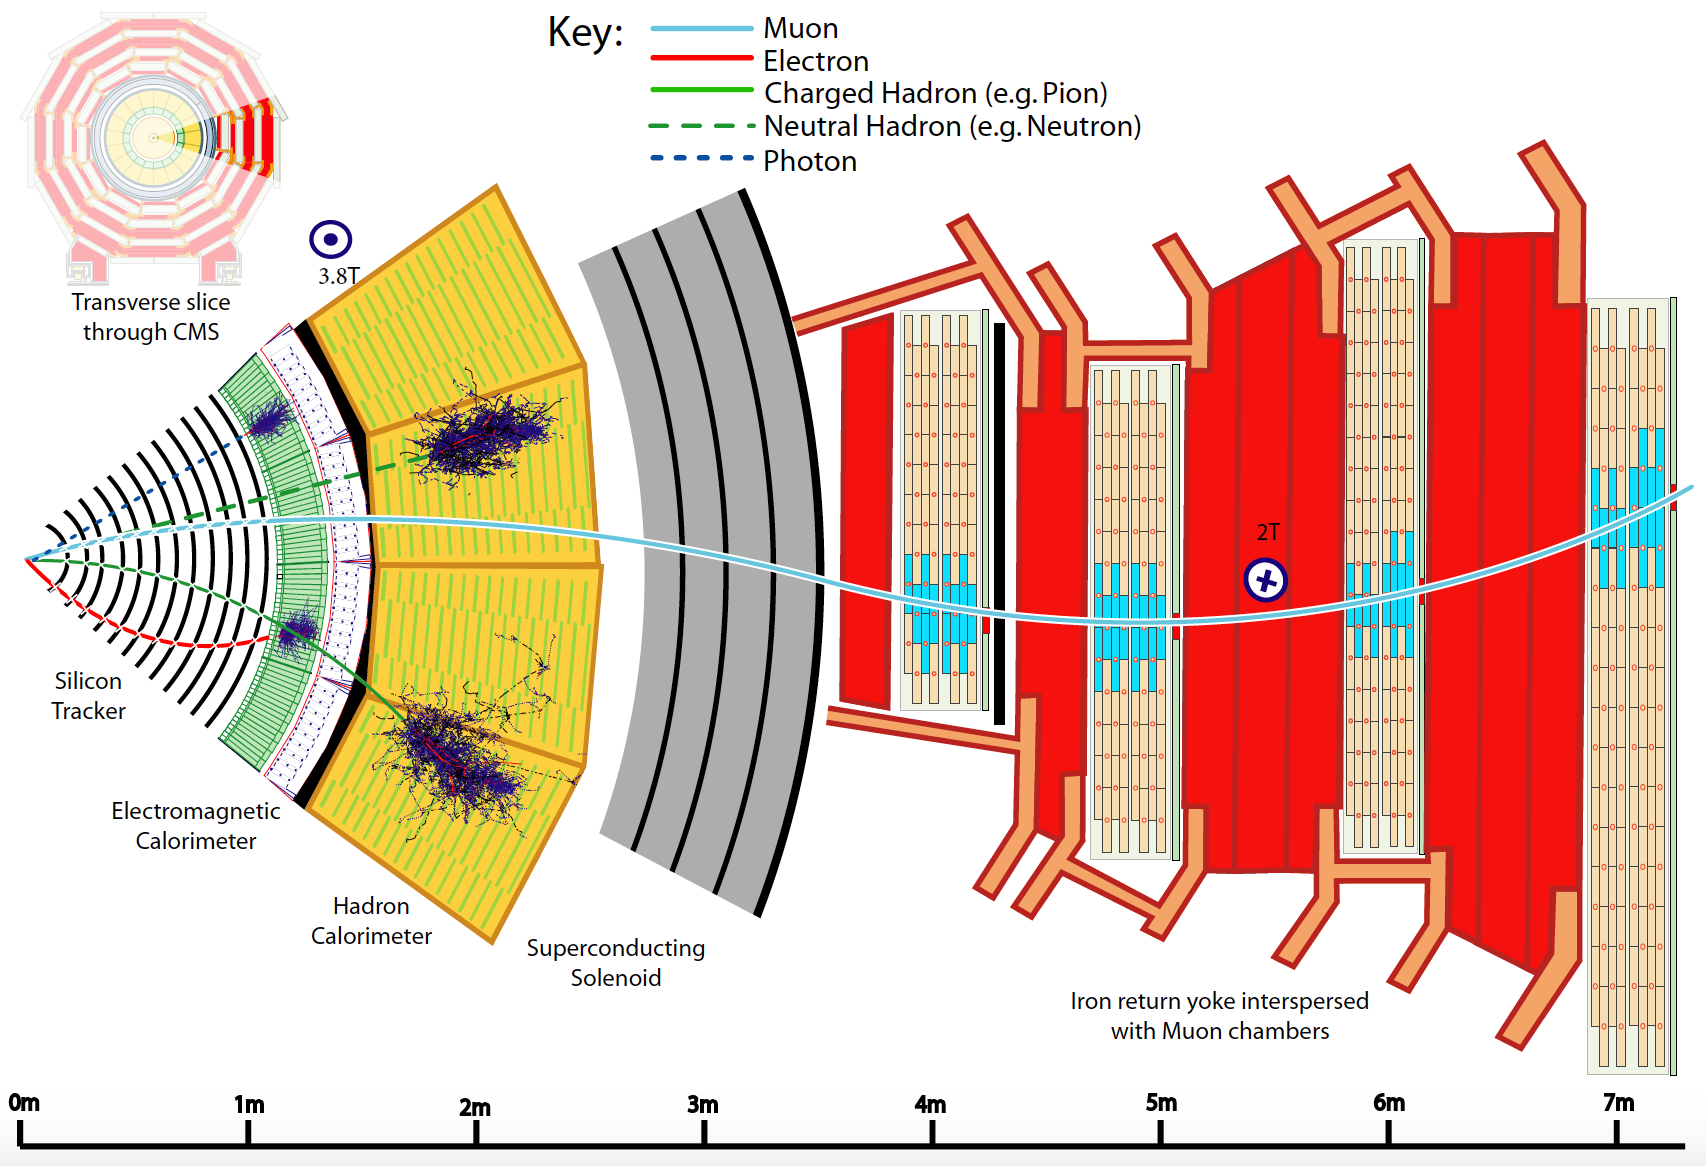
\includegraphics[width=0.75\textwidth]{figures/Transverse_slice_CMS.png}
    \caption[A transverse slice through the CMS detector with the main subsystems and components visible]{A transverse slice through the CMS detector with the main subsystems and components visible (figure obtained from Ref.~\citenum{CMS-PRF-14-001}). Several particles produced at the primary vertex and their interactions with the detector are also depicted.}
    \label{fig:detector_cms_transverse}
\end{figure}

\begin{figure}[htbp]
    \centering
    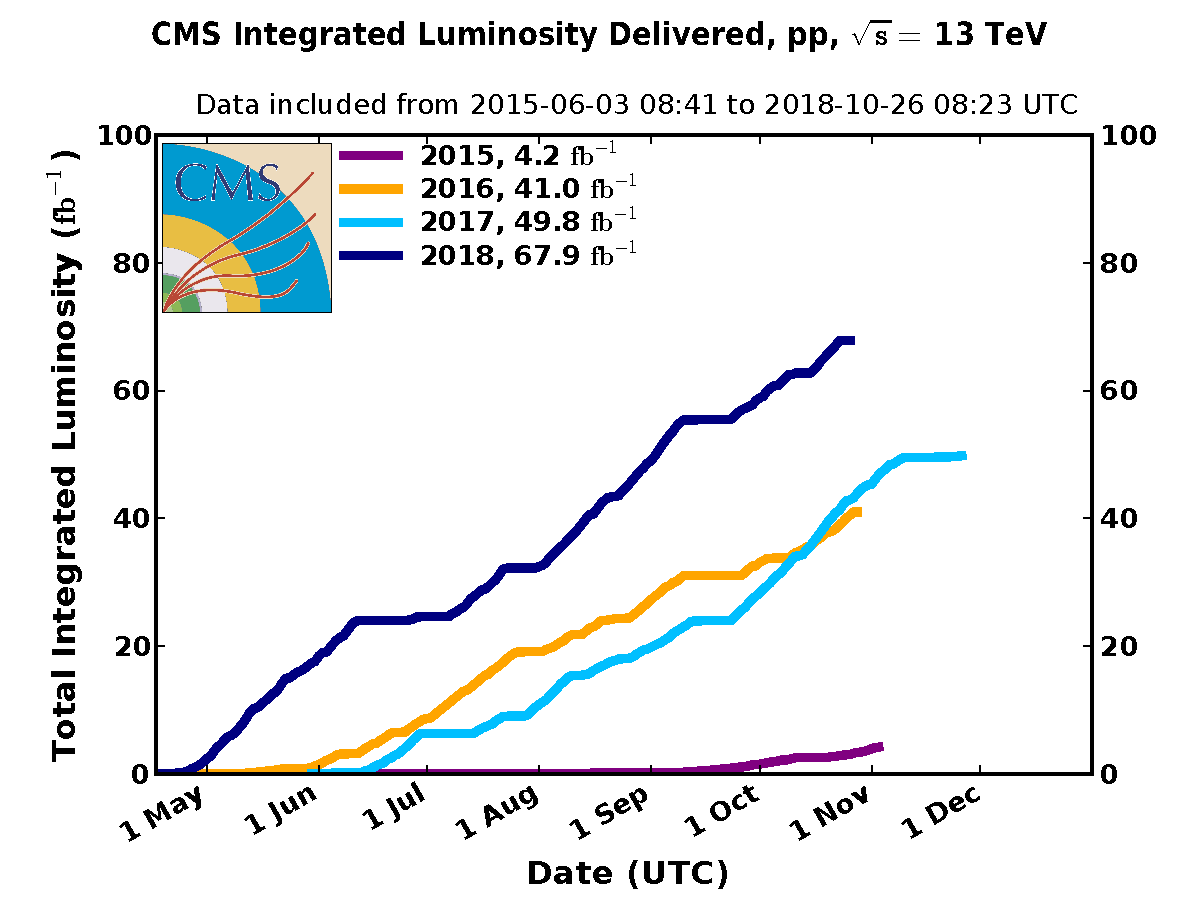
\includegraphics[width=0.75\textwidth]{figures/int_lumi_cumulative_pp_2_run2.pdf}
    \caption[The integrated luminosity of $\Pp\Pp$ collision data delivered to CMS during 2015 and Run-2 of the LHC]{The integrated luminosity of $\Pp\Pp$ collision data collected by CMS during 2015 and Run-2 of the LHC. Figure obtained from Ref.~\citenum{cmslumitwikipage}.}
    \label{fig:detector_cms_lumi}
\end{figure}

\begin{figure}[htbp]
    \centering
    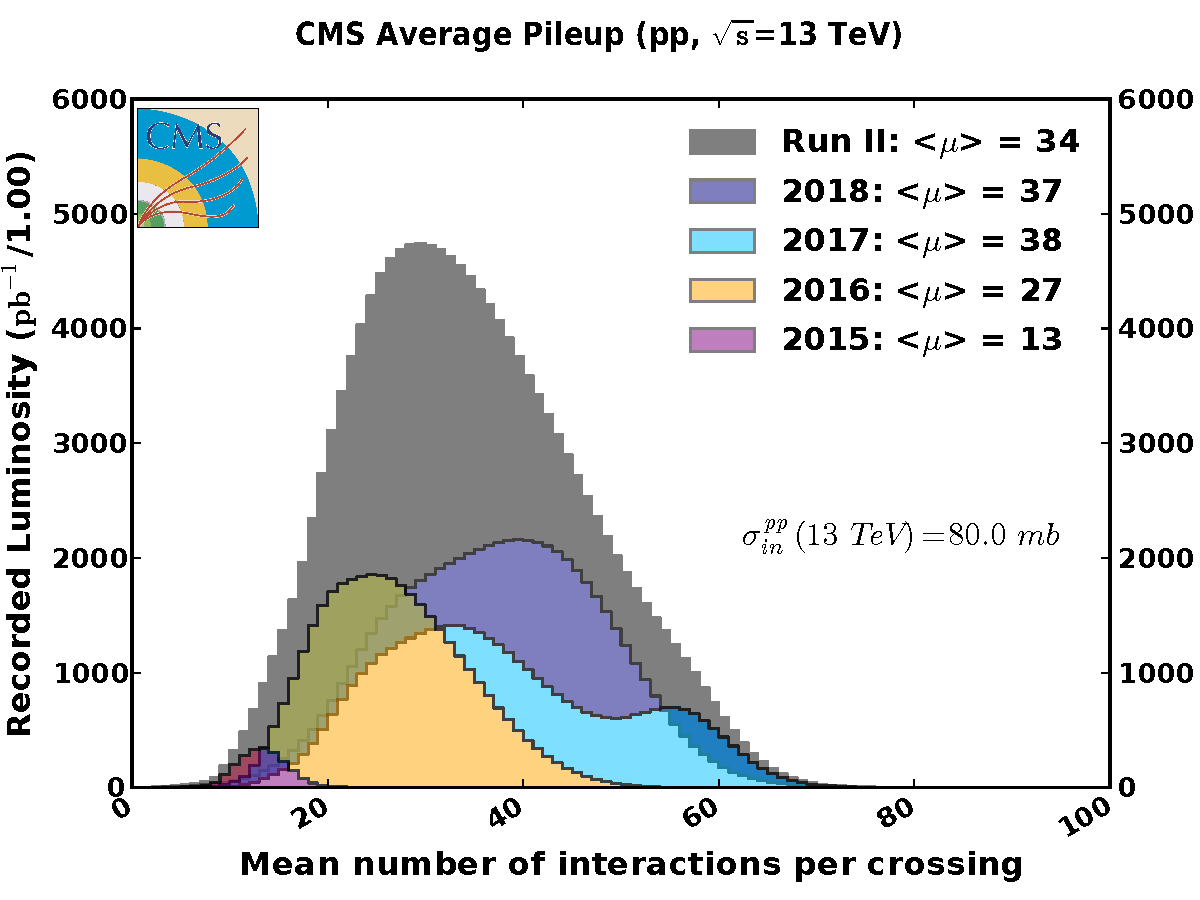
\includegraphics[width=0.75\textwidth]{figures/pileup_allYears_run2.pdf}
    \caption[The average number of pileup interactions at CMS during 2015 and Run-2 of the LHC]{The average number of pileup interactions at CMS during 2015 and Run-2 of the LHC. Figure obtained from Ref.~\citenum{cmslumitwikipage}.}
    \label{fig:detector_cms_pileup}
\end{figure}


\subsection{Jet energy corrections in the Level-1 Trigger}
\label{subsubsec:detector_jecs}

% Taken directly from second year report. Tidy up and improve. Can also look in Section 20 of my lab book for more info. Define what eta is, somewhere (can take from Section 14 of lab book)
\Gls{jec} are necessary to compensate for various losses when recording jet properties in the trigger. These losses depend on the transverse momentum \pt and pseudorapidity $\eta$. The calibrations ensure that the performance of the trigger is uniform across the detector. Firstly, some ideal (or reference) jets are needed to compare against given L1 jets. Since Monte Carlo datasets are used for the calibrations, the reference jets we use are the generator-level jets (or GenJets). These are stable, simulated particles clustered with the \gls{antikt} algorithm~\cite{Cacciari:2008gp} to form the jet. The state of these jets are post-hadronisation, before detector interaction. L1 jets need to be matched against the GenJets. From there, various studies can be performed such measuring the response ($< \ptsup{{\mathrm{L1}}} / \ptsup{{\mathrm{ref.}}} >$) of the detector, and its position and energy resolutions.

Once Calorimeter Layer-1 experts have derived scale factors for the physics objects, they are applied in Layer-2 where the calibrations are conducted. For jets, ntuples are created from the specified dataset and the L1 jets are matched to the GenJets using the variable $\Delta R$: 

\begin{equation}
\Delta R = \sqrt{\Delta \eta^2 + \Delta \phi^2}
\label{eq:delta_r}
\end{equation}

where $\phi$ is the azimuthal angle of the jet. The algorithm used to match the jets does so by inspecting each L1 jet in descending \pt and searching for a reference jet with $\Delta R < 0.25$. If there is more than one match, the reference jet with the smallest $\Delta R$ is taken. Then the next L1 jet (and so on) follows the same procedure, with the previous reference jet removed from the matching collection. Calibrations are then derived. The reciprocal of the response vs. $\ptsup{{\mathrm{L1}}}$ is plotted for each \abseta bin and correction curves are fitted to them (see Fig. \ref{fig:detector_jecs_corr_curves}). Once tuned such that the fit captures the low-\pt spike and high-\pt plateau, closure tests are conducted as the final step. The ntuples are remade with JECs and then matched with the reference jets to check that the calibrations have been properly applied. Plots such as Fig. \ref{fig:detector_jecs_scatter_BE} are then passed to the Trigger Studies Group to check over and continue the chain of trigger corrections and object calibrations.

\begin{figure}[htbp]
    \centering
    \begin{subfigure}[b]{0.45\textwidth}
        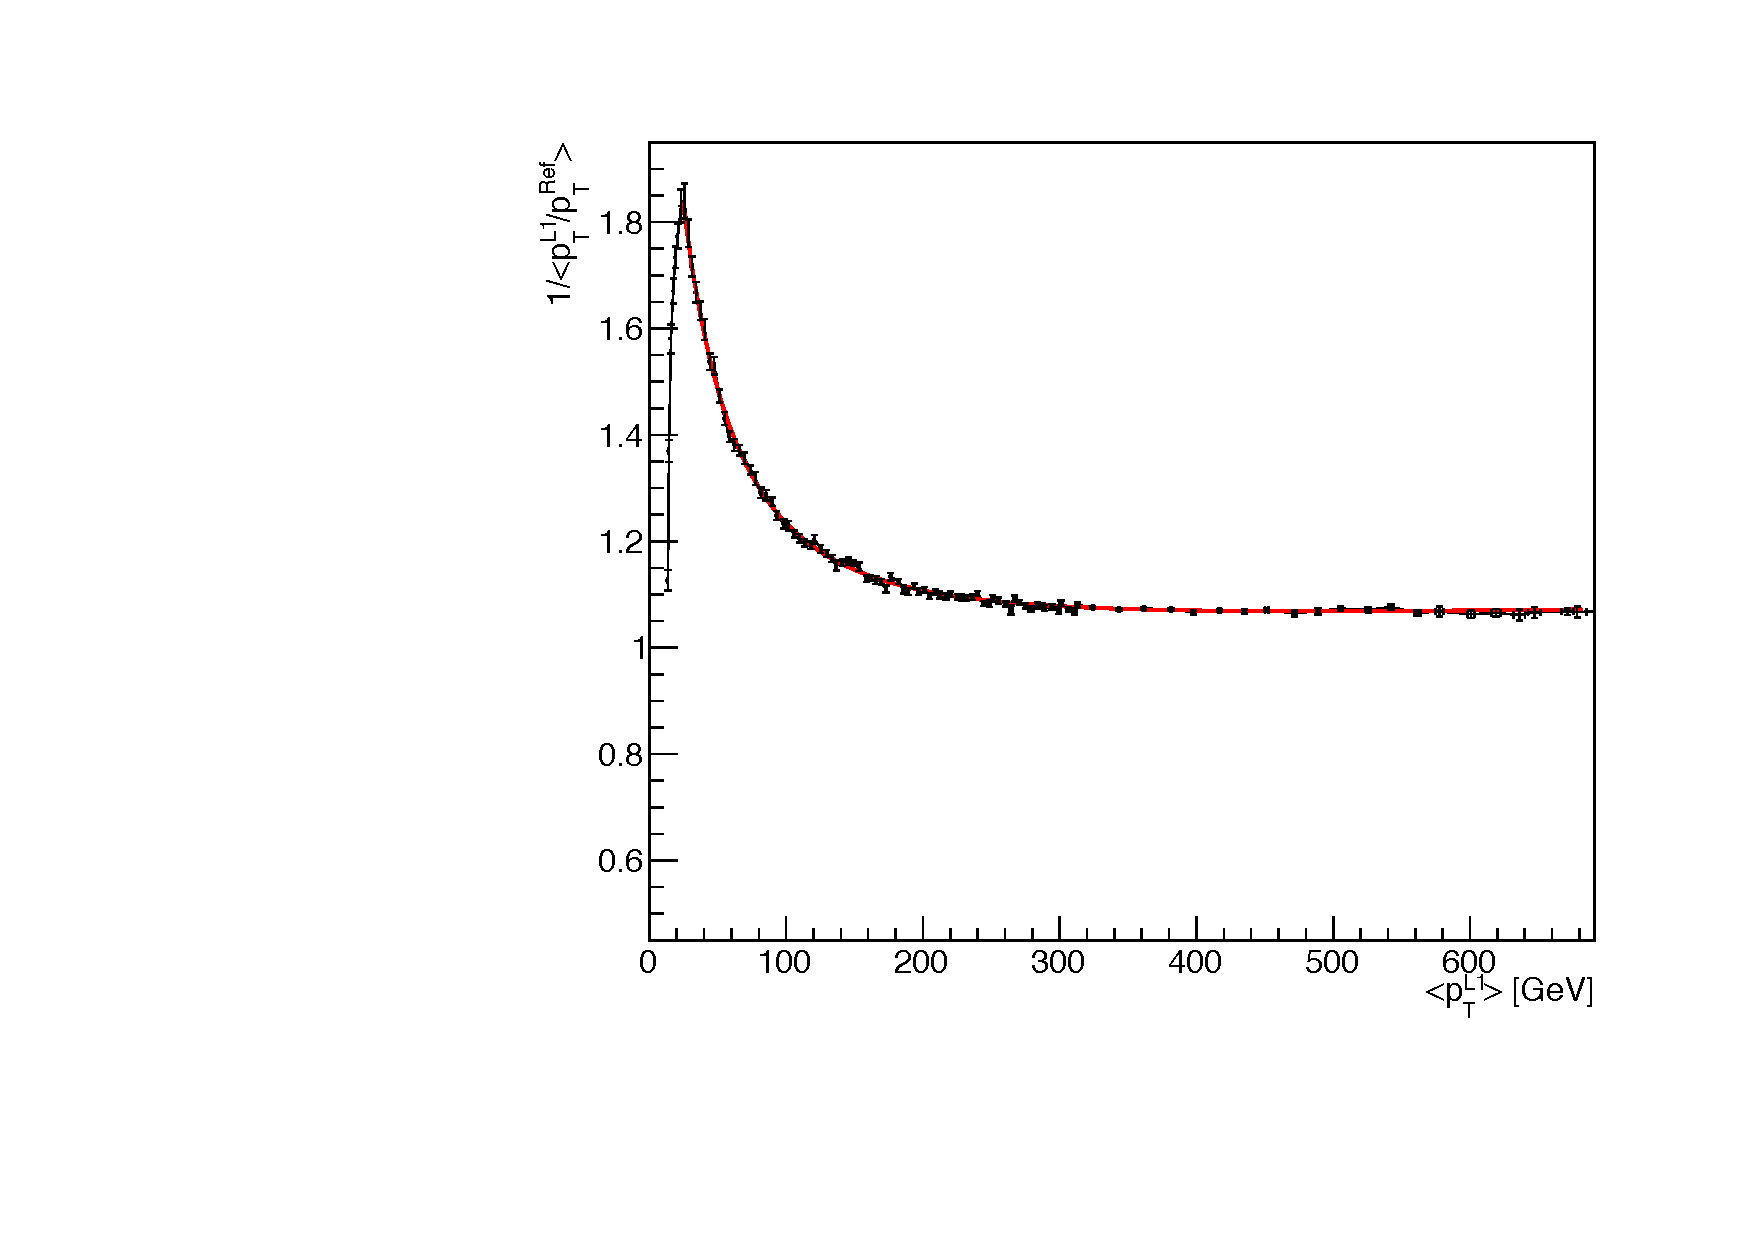
\includegraphics[width=\textwidth]{./figures/jecs//corrCurveBarrel.pdf}
        \caption{$0.435 < \abseta < 0.783$ (Barrel)}
        \label{fig:detector_jecs_corr_curve_Barrel}
    \end{subfigure}
    \hfill
    \begin{subfigure}[b]{0.45\textwidth}
        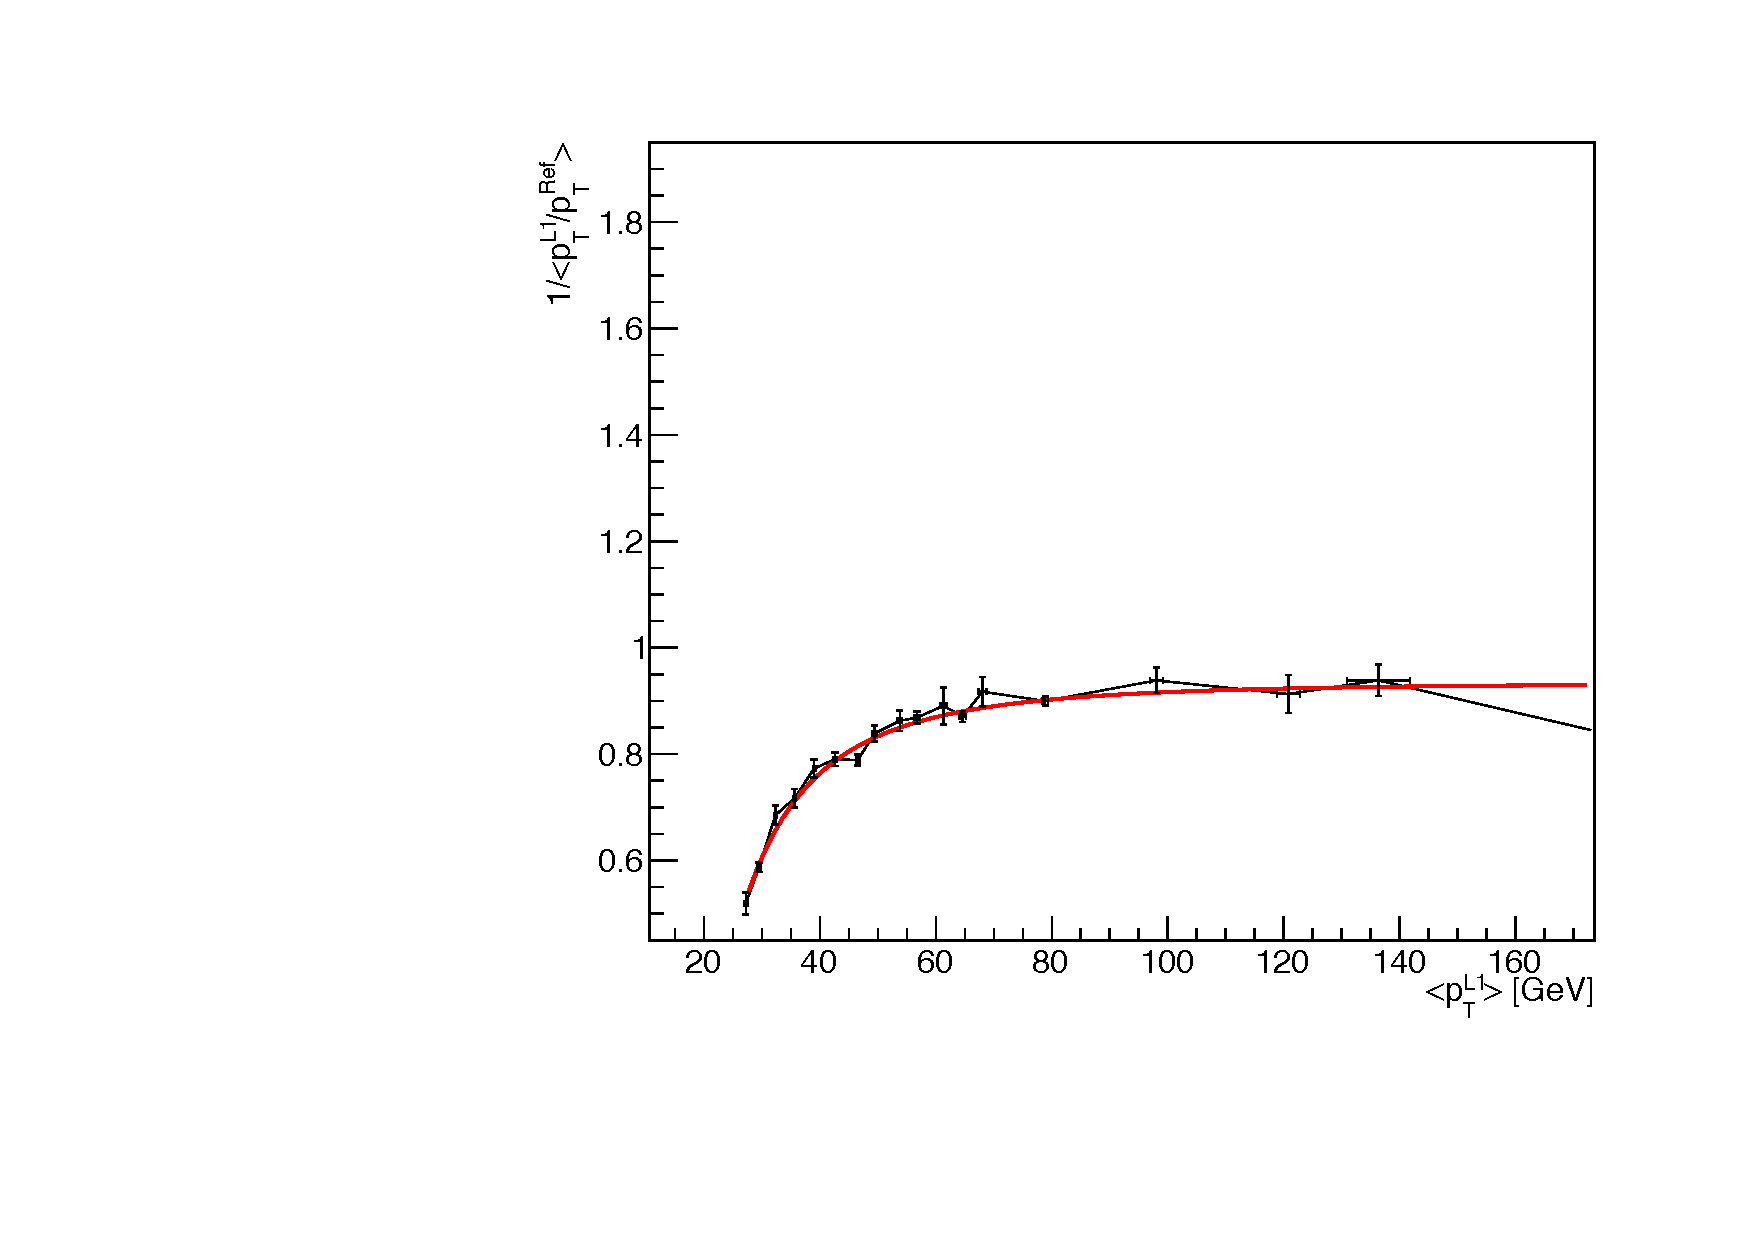
\includegraphics[width=\textwidth]{./figures/jecs/corrCurveHF.pdf}
        \caption{$4.191 < \abseta < 5.191$ (HF)}
        \label{fig:detector_jecs_corr_curve_HF}
    \end{subfigure}
\caption[Examples of correction curves used to calibrate the jet energies in two \abseta bins]{Examples of correction curves used to calibrate the jet energies in two \abseta bins. The response is plotted against the \pt of the Level-1 jet and a complex function produces a fit. These plots are from the jet energy corrections performed on 2018 QCD Monte Carlo.}
\label{fig:detector_jecs_corr_curves}
\end{figure}

\begin{figure}[htbp]
    \centering
    \begin{subfigure}[b]{0.45\textwidth}
        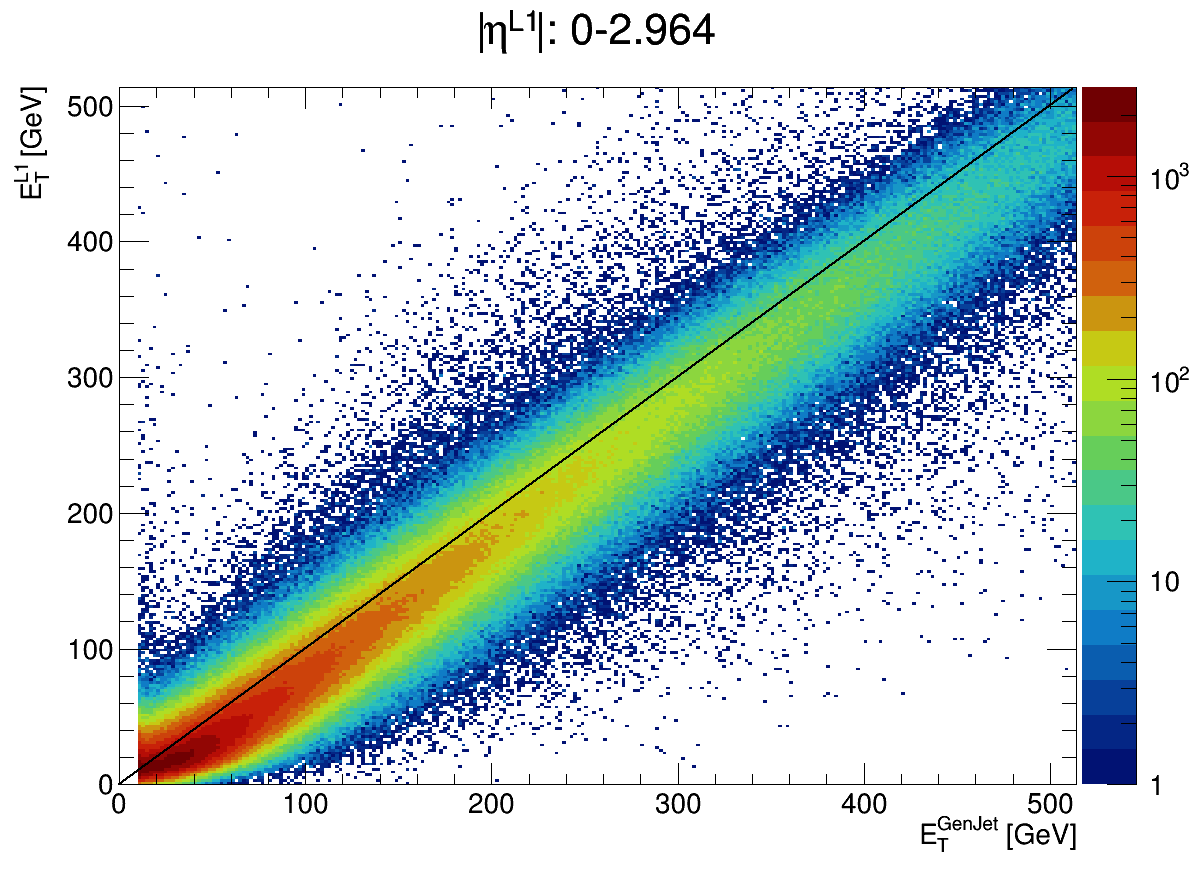
\includegraphics[width=\textwidth]{./figures/jecs/scatterPlotBeforeBE.png}
        \caption{Before corrections}
        \label{fig:detector_jecs_scatter_before_BE}
    \end{subfigure}
    \hfill
    \begin{subfigure}[b]{0.45\textwidth}
        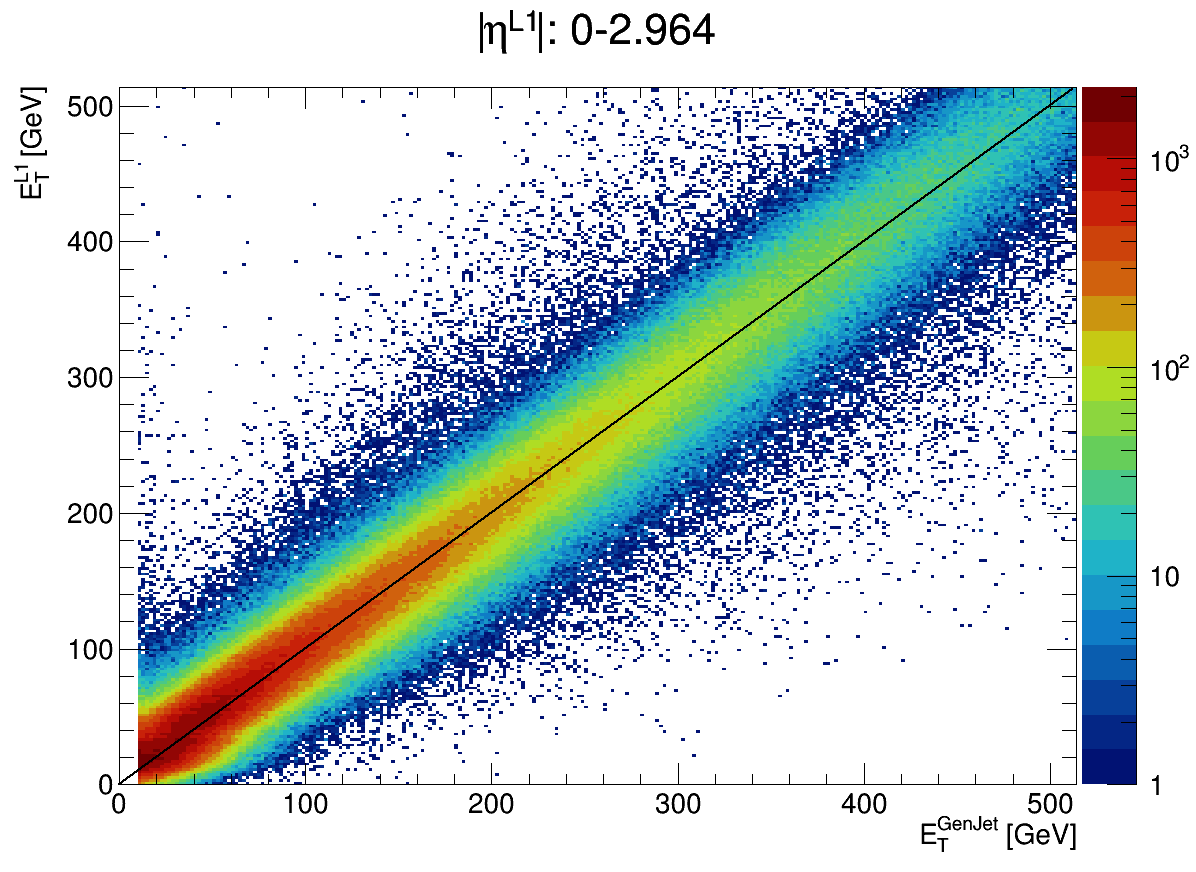
\includegraphics[width=\textwidth]{./figures/jecs/scatterPlotAfterBE.png}
        \caption{After corrections}
        \label{fig:detector_jecs_scatter_after_BE}
    \end{subfigure}
\caption[The energies of matched pairs of jets in the entire barrel and end cap, before and after jet energy corrections have been applied]{The energies of matched pairs of jets in the entire barrel and end cap, before and after jet energy corrections have been applied. After calibrations, the distribution is much more symmetrical. An equivalent plot using jets from LHC data is expected to look similar after applying these calibrations.}
\label{fig:detector_jecs_scatter_BE}
\end{figure}
